\documentclass[12pt,a4paper]{article}
\usepackage[T1]{fontenc}
\usepackage[utf8]{inputenc}
\usepackage{mathptmx}
\usepackage[indonesian]{babel}
\usepackage[a4paper,margin=2.5cm]{geometry}
\usepackage{setspace}
\usepackage{graphicx}
\usepackage{booktabs}
\usepackage{array}
\usepackage{float}
\usepackage{caption}
\usepackage{xcolor}
\usepackage{enumitem}
\usepackage[hidelinks]{hyperref}

\setstretch{1.4}
\setlength{\parindent}{0pt}
\setlength{\parskip}{0pt}
\setlength{\emergencystretch}{3em}
\hbadness=10000

% Underscore stabil untuk body text (di luar caption)
\newcommand{\db}[1]{\texttt{#1}}

% Nama database/tabel/fungsi ditulis apa adanya (tanpa underscore)
% supaya aman di caption.

\graphicspath{{../screenshot/}}

\usepackage{titlesec}
\titleformat{\section}{\normalfont\Large\bfseries}{\thesection}{1em}{}
\titleformat{\subsection}{\normalfont\large\bfseries}{\thesubsection}{1em}{}
\titlespacing*{\section}{0pt}{6pt}{2pt}
\titlespacing*{\subsection}{0pt}{5pt}{1pt}

\captionsetup{font=small,labelfont=bf,justification=centering}

\begin{document}

% ============================ COVER ============================
\begin{titlepage}
\thispagestyle{empty}
\begin{center}

\textbf{\large\MakeUppercase{Laporan Praktikum Pemrograman Basis Data \\ Week 5: Fungsi pada Basis Data (PostgreSQL)}}

\vspace{1.2cm}

\textbf{\MakeUppercase{Laporan Praktikum}}

\vspace{2cm}


\includegraphics[width=4.5cm,height=4.5cm,keepaspectratio]{assets/logo-unesa.png}

\vspace{2cm}

Oleh\\[0.3cm]
\textbf{MUHROMIN}\\[0.1cm]
\textbf{NIM 25051214046}

\vfill

\textbf{UNIVERSITAS NEGERI SURABAYA}\\[0.2cm]
\textbf{FAKULTAS TEKNIK}\\[0.2cm]
\textbf{PROGRAM STUDI S1 SISTEM INFORMASI}\\[0.2cm]
\textbf{2026}

\end{center}
\end{titlepage}

% ============================ ISI ============================

\section*{Ringkasan Praktikum}
\smallskip
Praktikum ini membahas pembuatan dan pemanfaatan fungsi (stored function) pada basis data, meliputi fungsi skalar murni, fungsi yang membaca tabel, penerapan dalam skenario nyata, pengujian, penelusuran galat, dan pengukuran kinerja.

Seluruh praktikum dijalankan pada PostgreSQL 18 dengan basis data kerja db\_fungsi\_hr. Soal aslinya ditulis untuk MySQL sehingga dilakukan penyesuaian sintaks. Data diambil dari dataset employees melalui foreign table, dengan rincian sebagai berikut

\begin{center}
\begin{tabular}{|l|c|c|c|c|}
\hline
\textbf{departemen} & \textbf{pegawai} & \textbf{penempatan} & \textbf{gaji} & \textbf{uji\_fungsi}\\
\hline
9 & 5.000 & 5.524 & 47.603 & 16\\
\hline
\end{tabular}
\end{center}

\section*{A. Persiapan}

\begin{figure}[H]
\centering
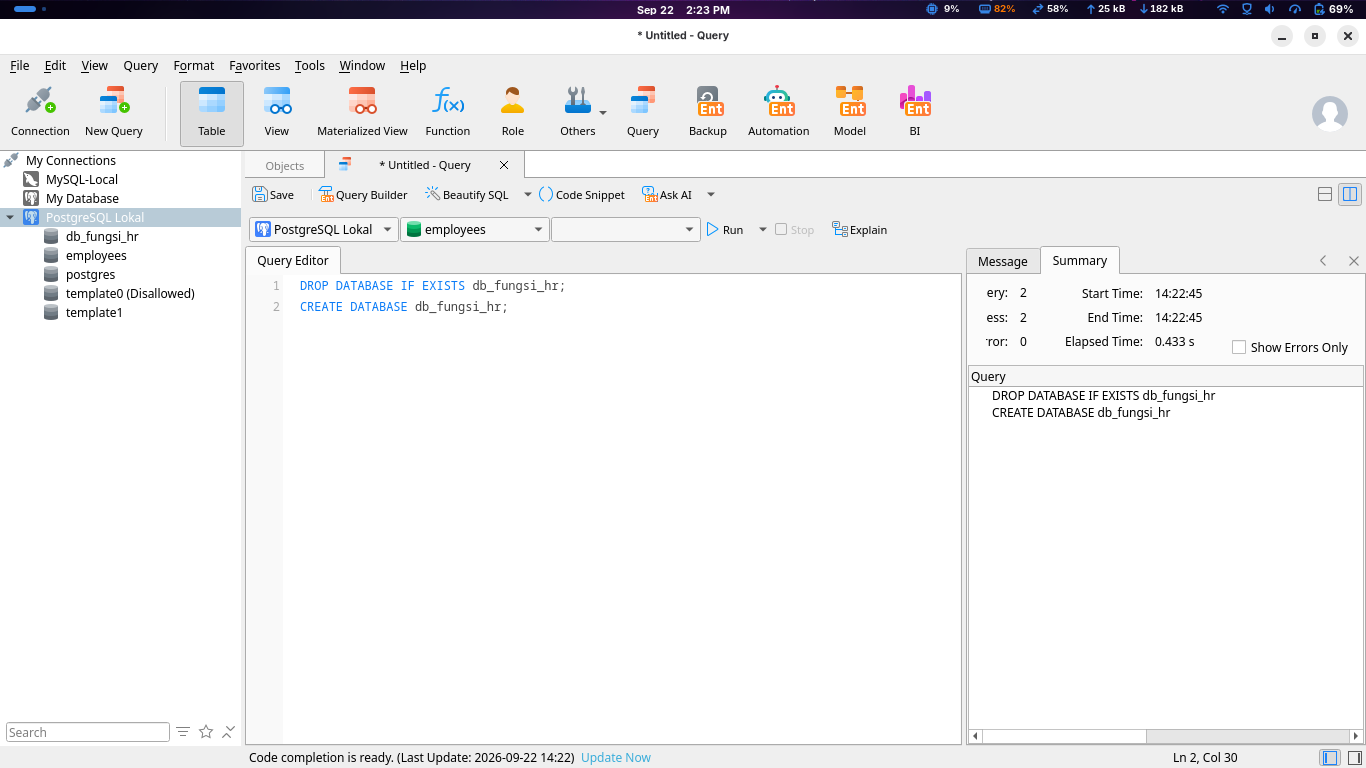
\includegraphics[width=0.9\textwidth,keepaspectratio]{ss_01_create_db.png.png}
\caption{Database db\_fungsi\_hr berhasil dibuat.}
\end{figure}
\smallskip
Dibuat database kerja sebagai tempat seluruh objek praktikum.

\begin{figure}[H]
\centering
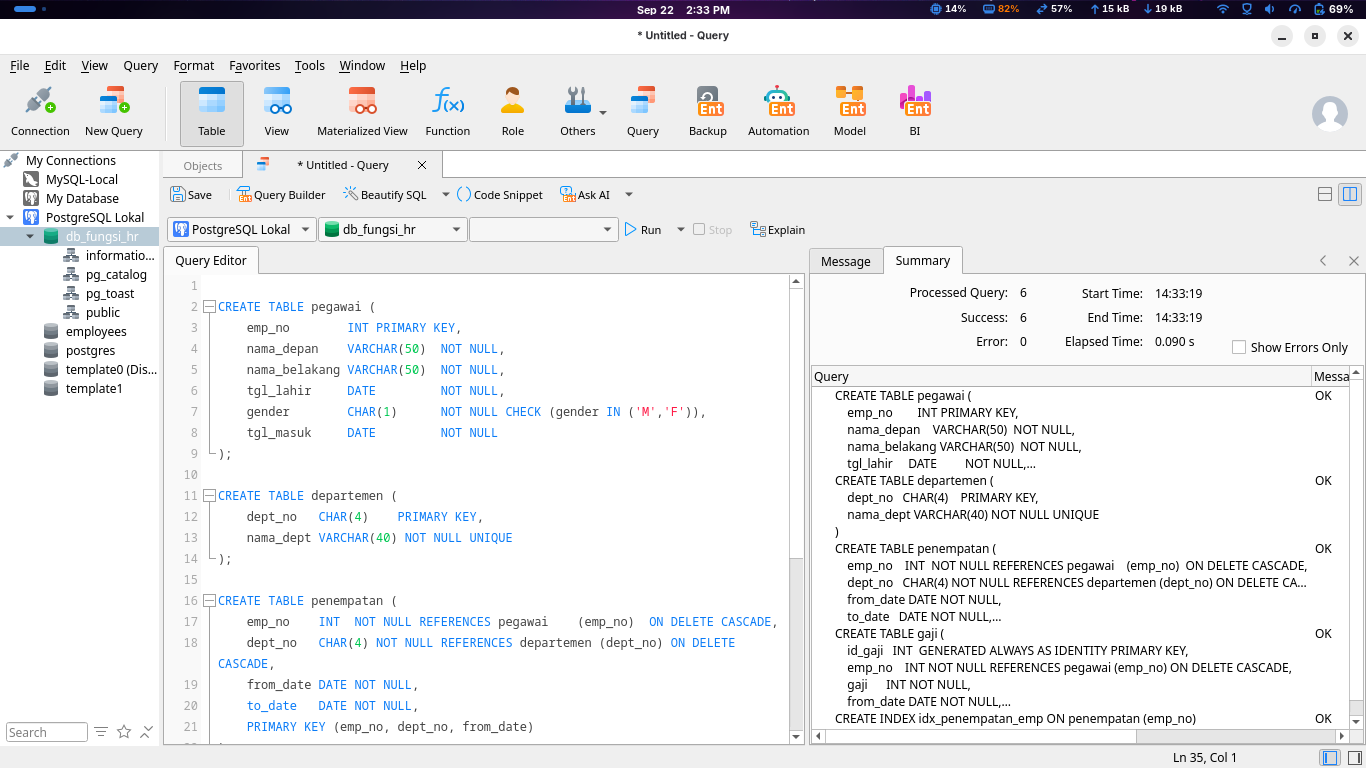
\includegraphics[width=0.9\textwidth,keepaspectratio]{ss_02_tabel.png}
\caption{Keempat tabel operasional berhasil dibuat.}
\end{figure}
\smallskip
Empat tabel operasional dibuat, yaitu pegawai, departemen, penempatan, dan gaji, lengkap dengan kunci utama, kunci asing, dan indeks.

\begin{figure}[H]
\centering
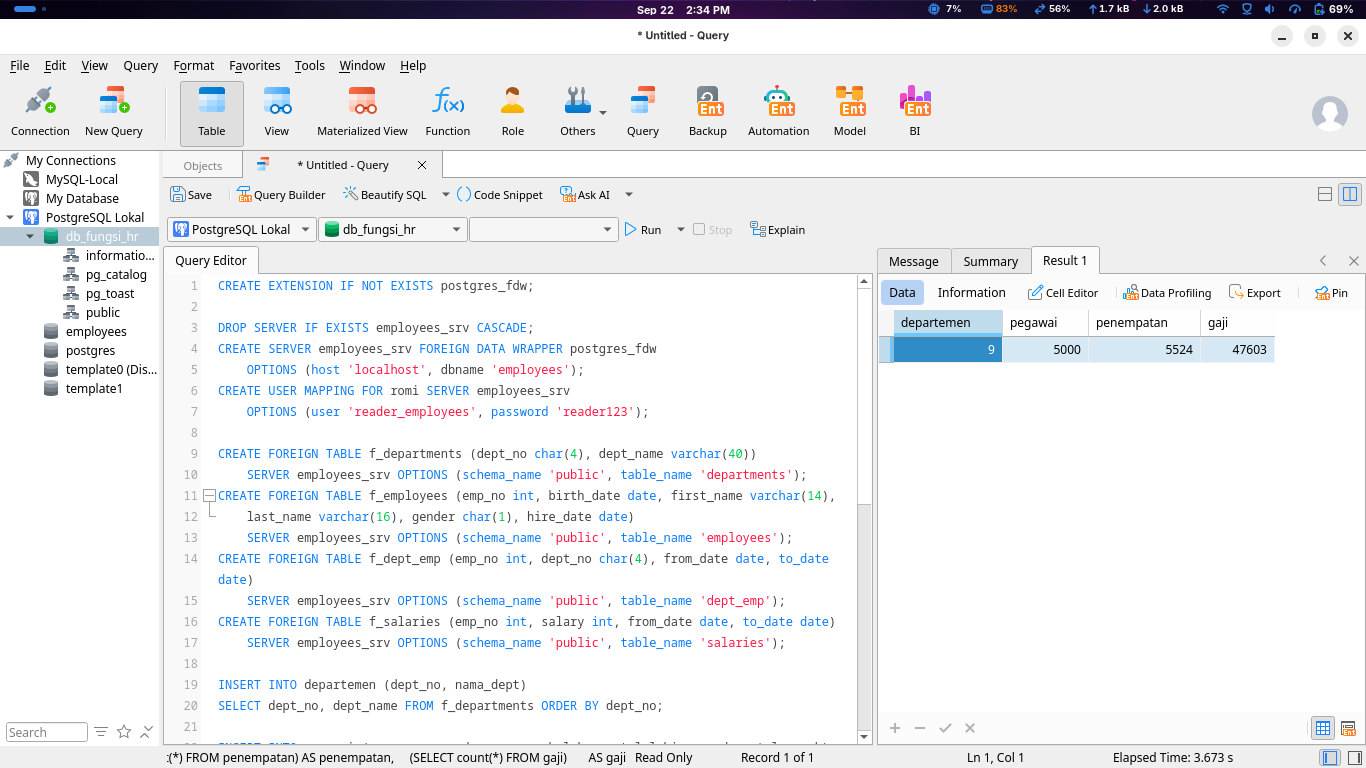
\includegraphics[width=0.9\textwidth,keepaspectratio]{ss_03_jumlah_baris.png}
\caption{Jumlah baris keempat tabel setelah pengisian data.}
\end{figure}
\smallskip
Data diisi dari database employees melalui foreign table (postgres\_fdw).

\begin{figure}[H]
\centering
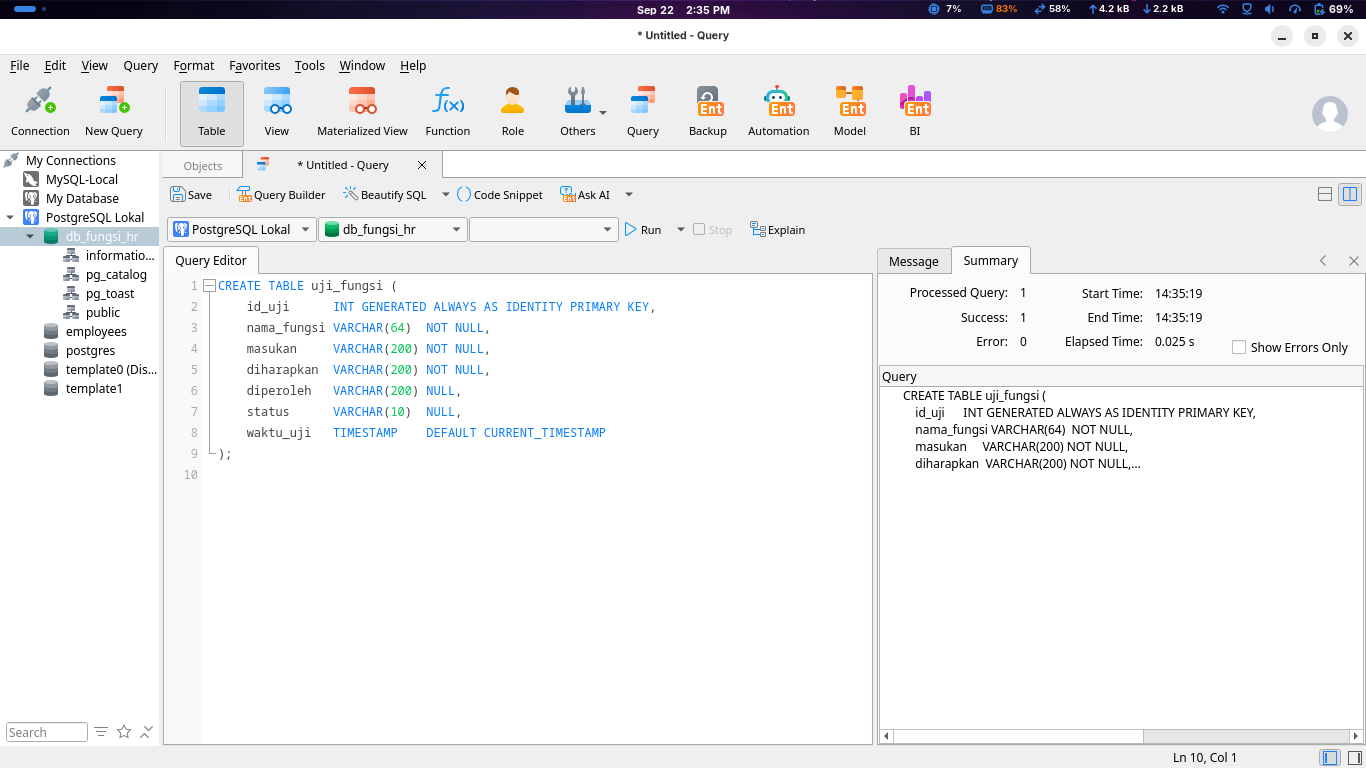
\includegraphics[width=0.9\textwidth,keepaspectratio]{ss_04_uji_fungsi_table.png}
\caption{Tabel uji\_fungsi berhasil dibuat.}
\end{figure}
\smallskip
Tabel pendukung untuk mencatat hasil pengujian terpusat.

\section*{B. Fungsi Skalar Murni}

\begin{figure}[H]
\centering
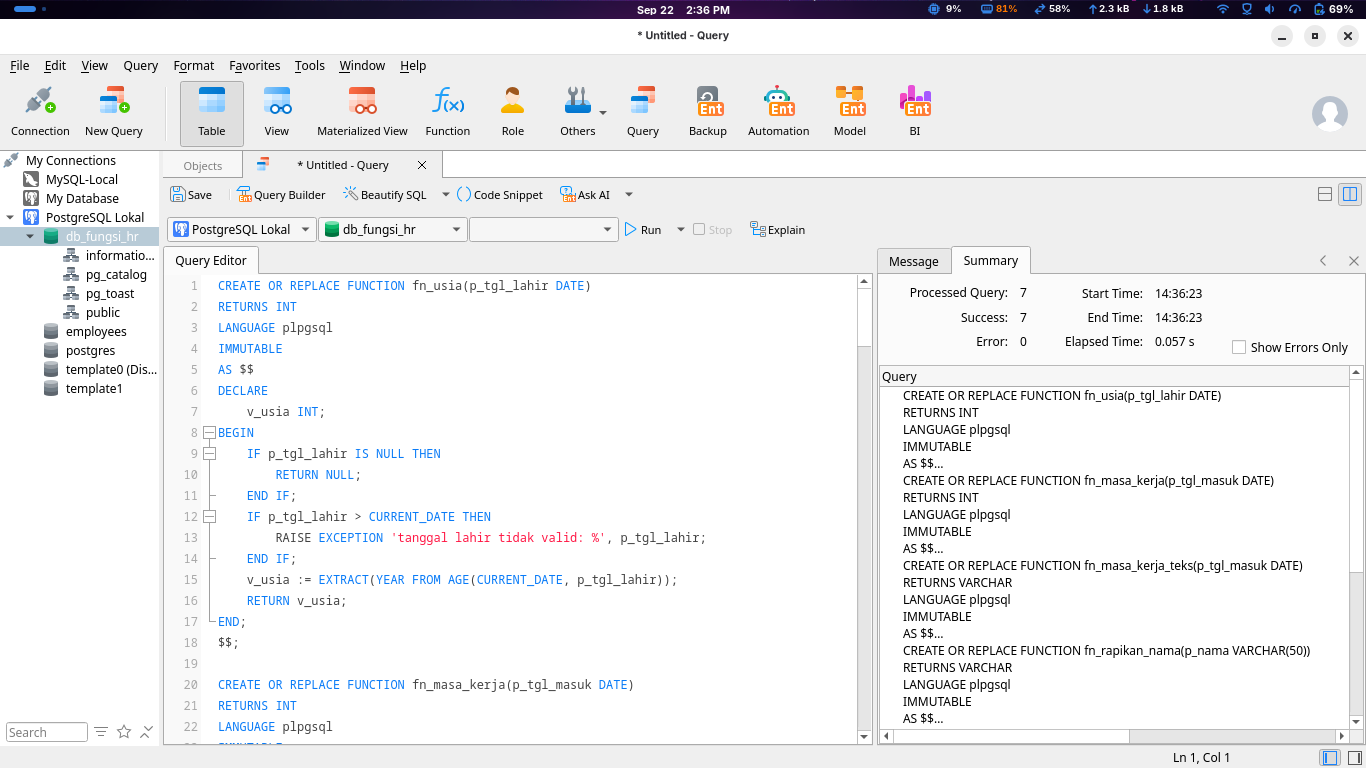
\includegraphics[width=0.9\textwidth,keepaspectratio]{ss_05_fungsi_B.png}
\caption{Enam fungsi skalar murni berhasil dibuat.}
\end{figure}
\smallskip
Enam fungsi dibuat, yaitu fn\_usia, fn\_masa\_kerja, fn\_masa\_kerja\_teks, fn\_rapikan\_nama, fn\_format\_rupiah, dan fn\_kategori\_gaji. Fungsi ini tidak menyentuh tabel, dan hasilnya dihitung dari parameter.

\begin{figure}[H]
\centering
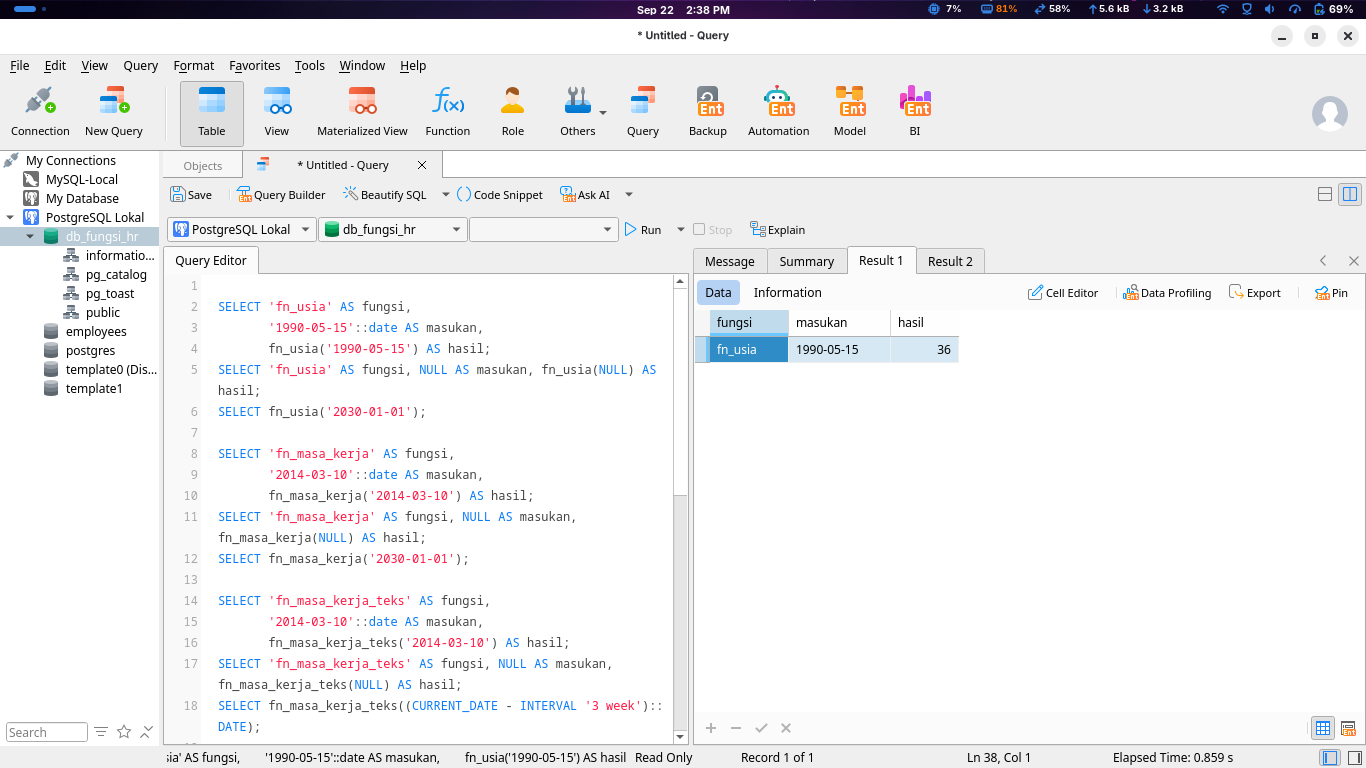
\includegraphics[width=0.9\textwidth,keepaspectratio]{ss_06_uji_B.png}
\caption{Hasil pengujian fungsi Bagian B (termasuk penolakan input tak valid).}
\end{figure}
\smallskip
Setiap fungsi diuji dengan nilai normal, NULL, dan nilai tidak wajar (tanggal masa depan, gaji negatif). Fungsi mengembalikan NULL untuk input NULL dan menolak input tak valid dengan RAISE EXCEPTION.

\textbf{Analisis:} fn\_usia bergantung pada CURRENT\_DATE sehingga hasilnya berubah seiring waktu. Bila dipaksa IMMUTABLE, mesin basis data boleh meng-cache hasilnya sehingga pada replikasi node akan menampilkan usia yang usang, dan hasil query yang disimpan sementara (view materialized) akan membeku. Maka fungsi ini tidak boleh dideklarasikan IMMUTABLE.

\section*{C. Fungsi yang Membaca Tabel}

\begin{figure}[H]
\centering
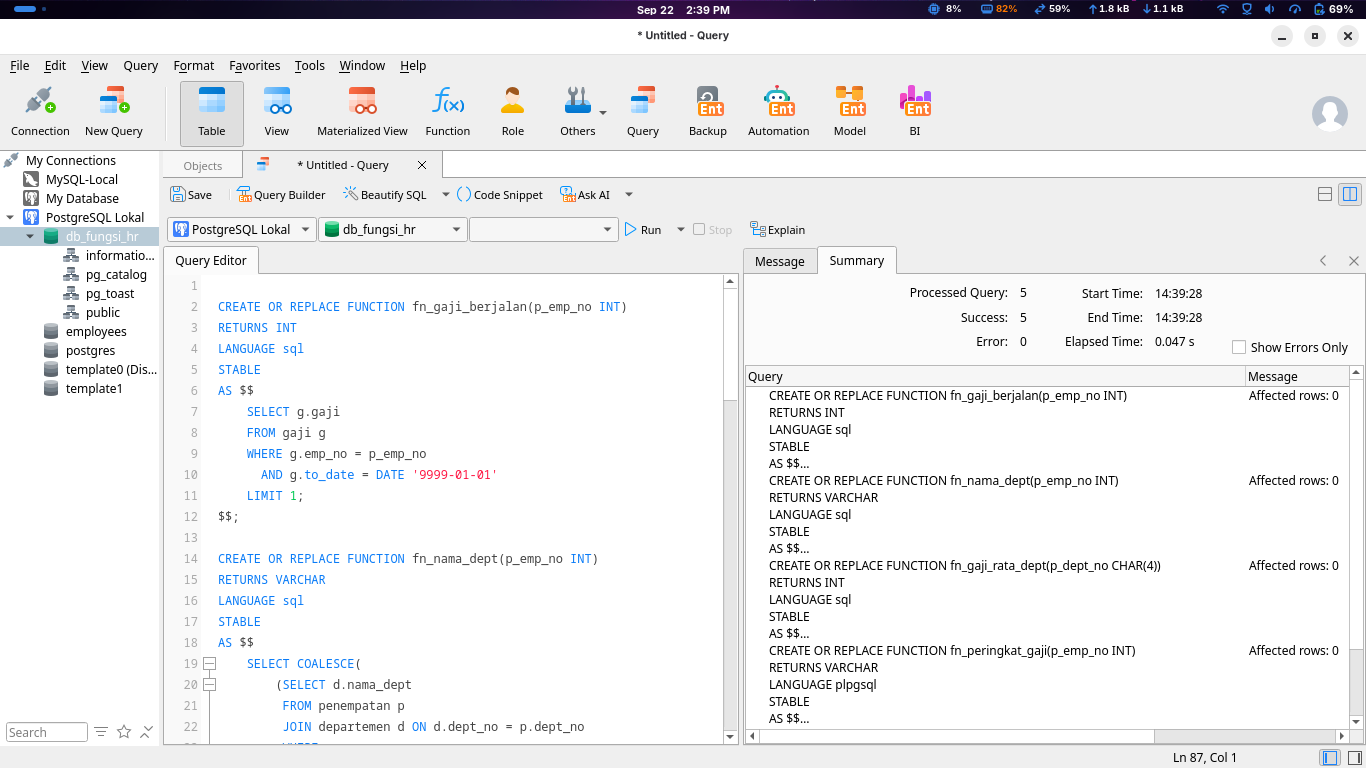
\includegraphics[width=0.9\textwidth,keepaspectratio]{ss_07_fungsi_C.png}
\caption{Lima fungsi pembaca tabel berhasil dibuat.}
\end{figure}
\smallskip
Lima fungsi STABLE yang membaca tabel, yaitu fn\_gaji\_berjalan, fn\_nama\_dept, fn\_gaji\_rata\_dept, fn\_peringkat\_gaji, serta fn\_total\_naik.

\begin{figure}[H]
\centering
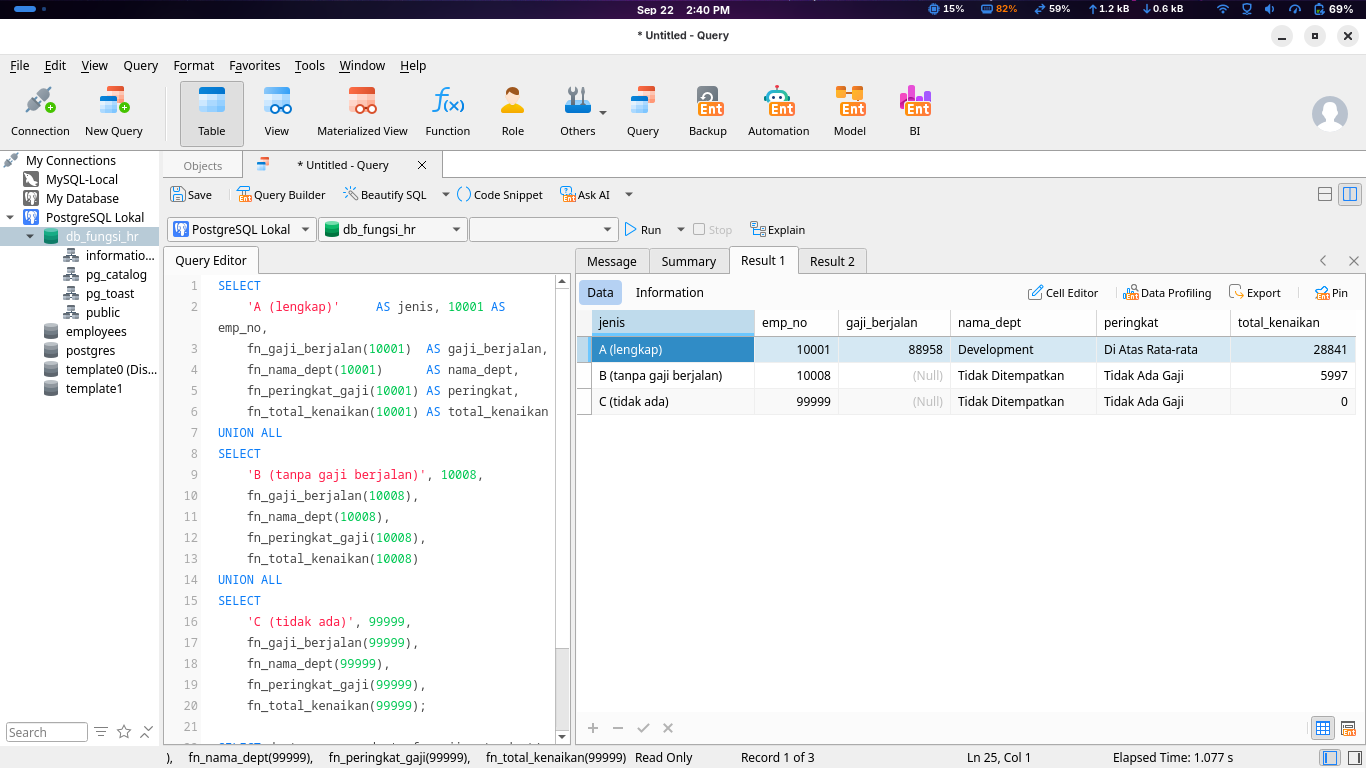
\includegraphics[width=0.9\textwidth,keepaspectratio]{ss_08_uji_C.png}
\caption{Pengujian fungsi Bagian C dengan tiga jenis masukan.}
\end{figure}
\smallskip
Fungsi diuji dengan tiga jenis emp\_no, yaitu (A) data lengkap, (B) ada pegawai tetapi tanpa gaji berjalan, dan (C) pegawai tidak ada.

\textbf{Analisis:} Penyusunan fungsi secara berlapis memberi reuse dan konsistensi (logika ditulis sekali, dipakai di mana saja) serta keterbacaan dan pemeliharaan (query laporan pendek, aturan cukup diubah di satu tempat). Risikonya, kinerja dan ketergantungan berantai, yaitu tiap lapisan menambah panggilan sehingga memperlambat, dan perubahan/penghapusan fungsi dasar berdampak kaskade ke semua pemanggil.

\section*{D. Penerapan dalam Skenario Nyata}

\subsection*{D1. Laporan Profil Pegawai}
\begin{figure}[H]
\centering
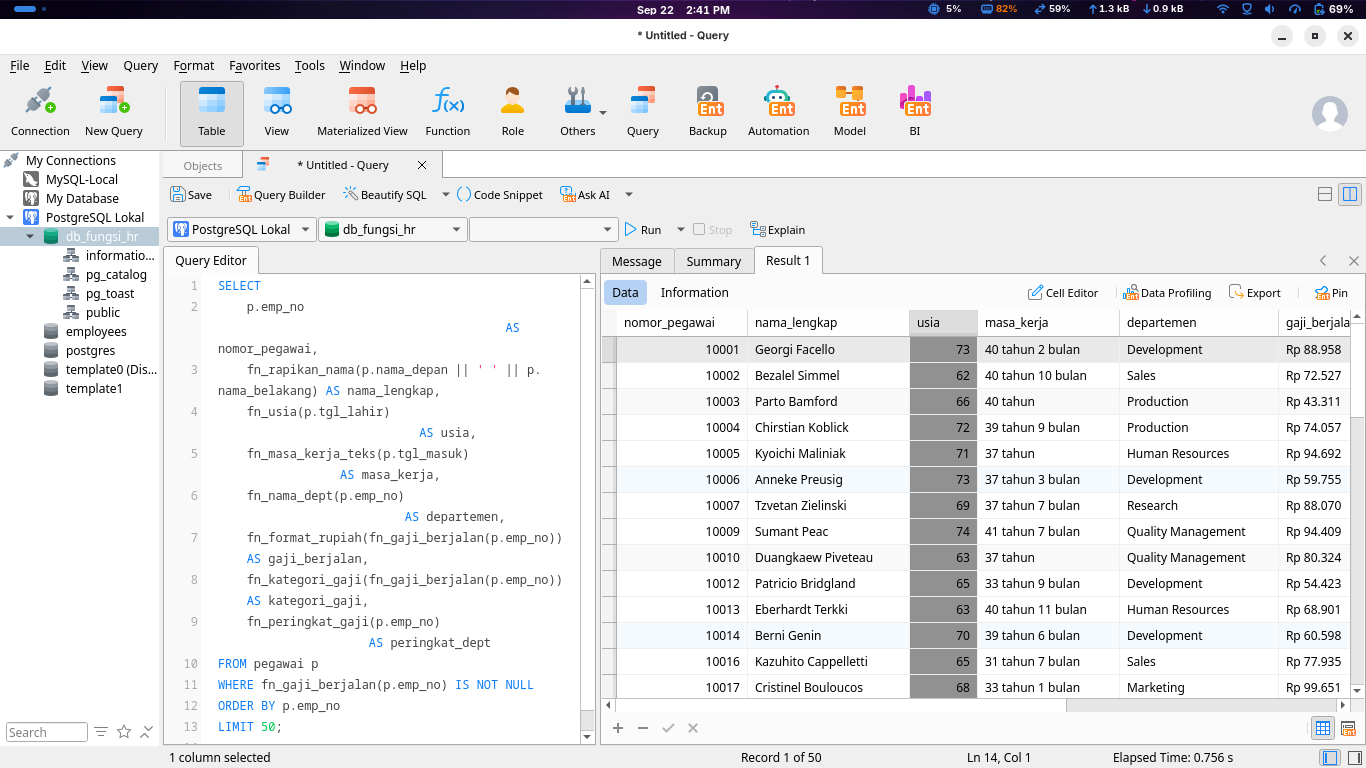
\includegraphics[width=0.95\textwidth,keepaspectratio]{ss_09_D1_profil.png}
\caption{Laporan profil pegawai (D1).}
\end{figure}
\smallskip
Laporan 50 baris, dan seluruh kolom turunan berasal dari pemanggilan fungsi.

\subsection*{D2. Proyeksi Pensiun}
\begin{figure}[H]
\centering
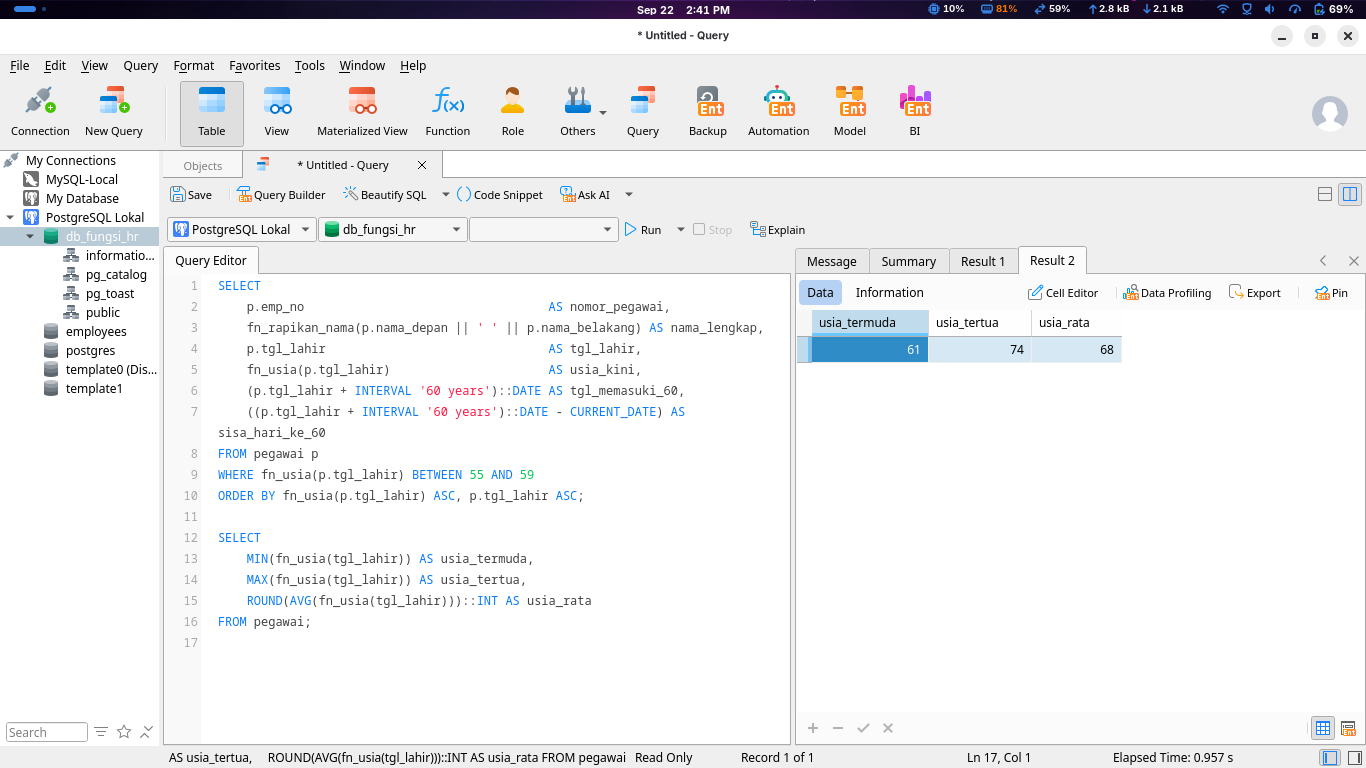
\includegraphics[width=0.9\textwidth,keepaspectratio]{ss_10_D2_pensiun.png}
\caption{Proyeksi pensiun (D2), 0 baris karena seluruh pegawai sudah lebih dari 60 tahun}
\end{figure}
\smallskip
Query memakai fn\_usia di WHERE dan ORDER BY. Pada dataset ini seluruh pegawai sudah berusia di atas 60 tahun sehingga hasil 0 baris, dan temuan ini dilaporkan apa adanya.

\subsection*{D3. Rekap per Departemen}
\begin{figure}[H]
\centering
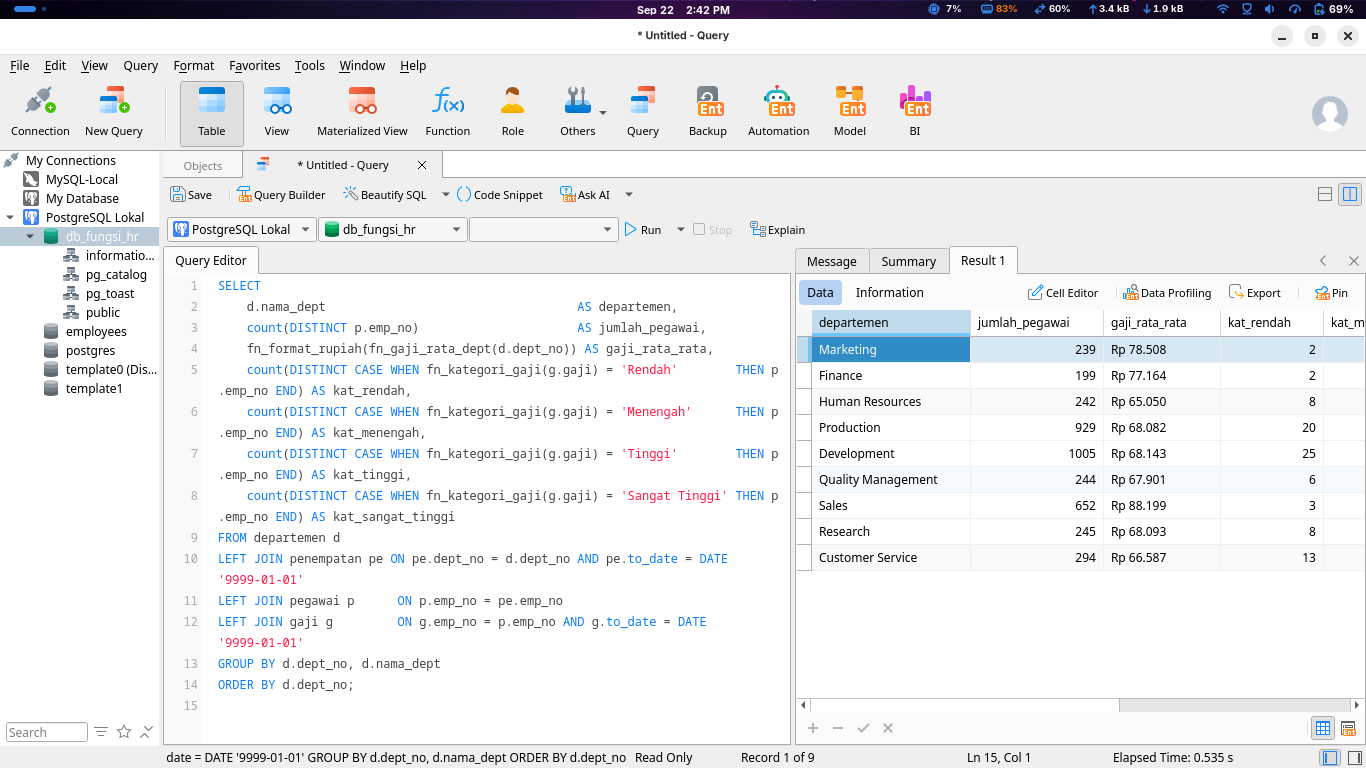
\includegraphics[width=0.95\textwidth,keepaspectratio]{ss_11_D3_rekap.png}
\caption{Rekapitulasi per departemen (D3).}
\end{figure}
\smallskip
Rekapitulasi per departemen meliputi jumlah pegawai, gaji rata-rata (rupiah), dan sebaran kategori gaji.

\subsection*{D4. Validasi Gaji}
\begin{figure}[H]
\centering
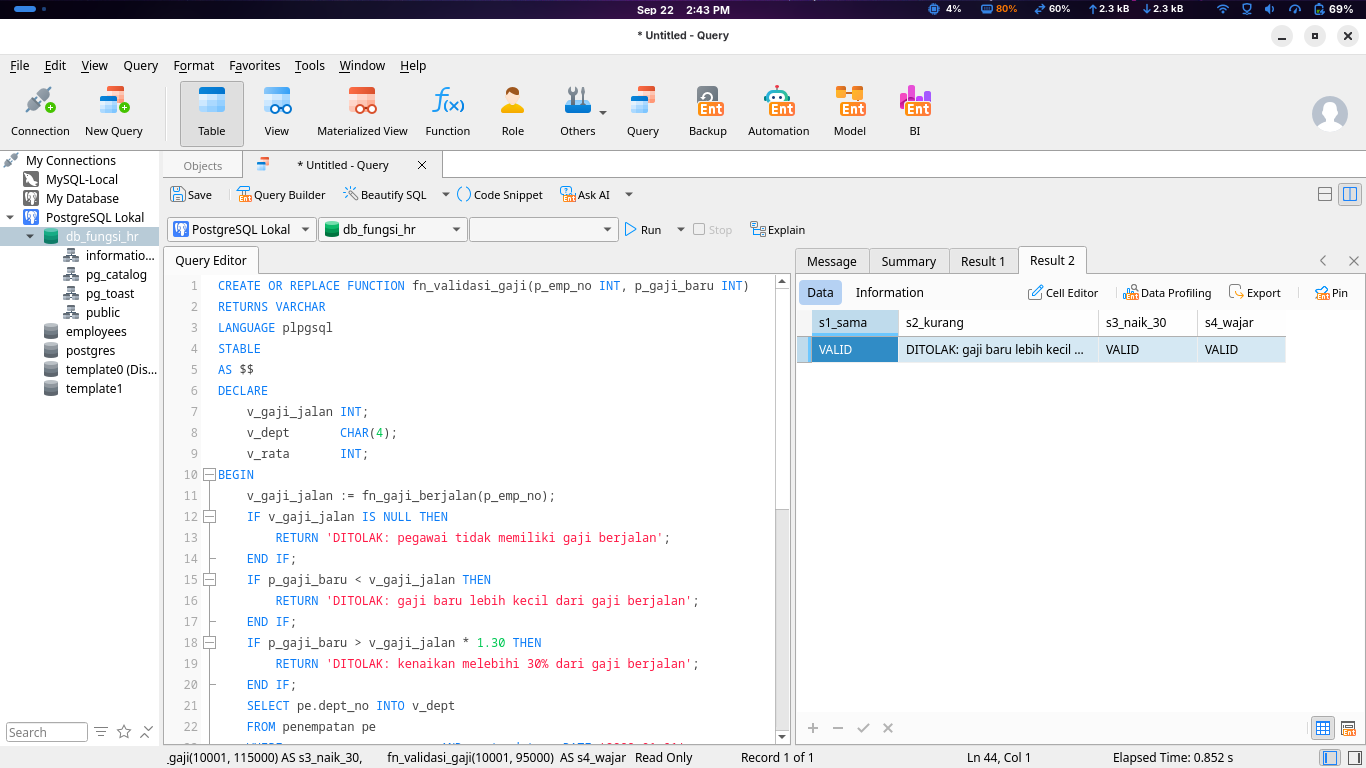
\includegraphics[width=0.9\textwidth,keepaspectratio]{ss_12_D4_validasi.png}
\caption{Hasil validasi gaji beberapa skenario (D4).}
\end{figure}
\smallskip
fn\_validasi\_gaji mengembalikan VALID atau pesan penolakan (gaji baru kurang dari berjalan, kenaikan lebih dari 30\%, atau lebih dari 2 kali rata-rata departemen).

\subsection*{D5. Trigger Validasi Gaji}
\begin{figure}[H]
\centering
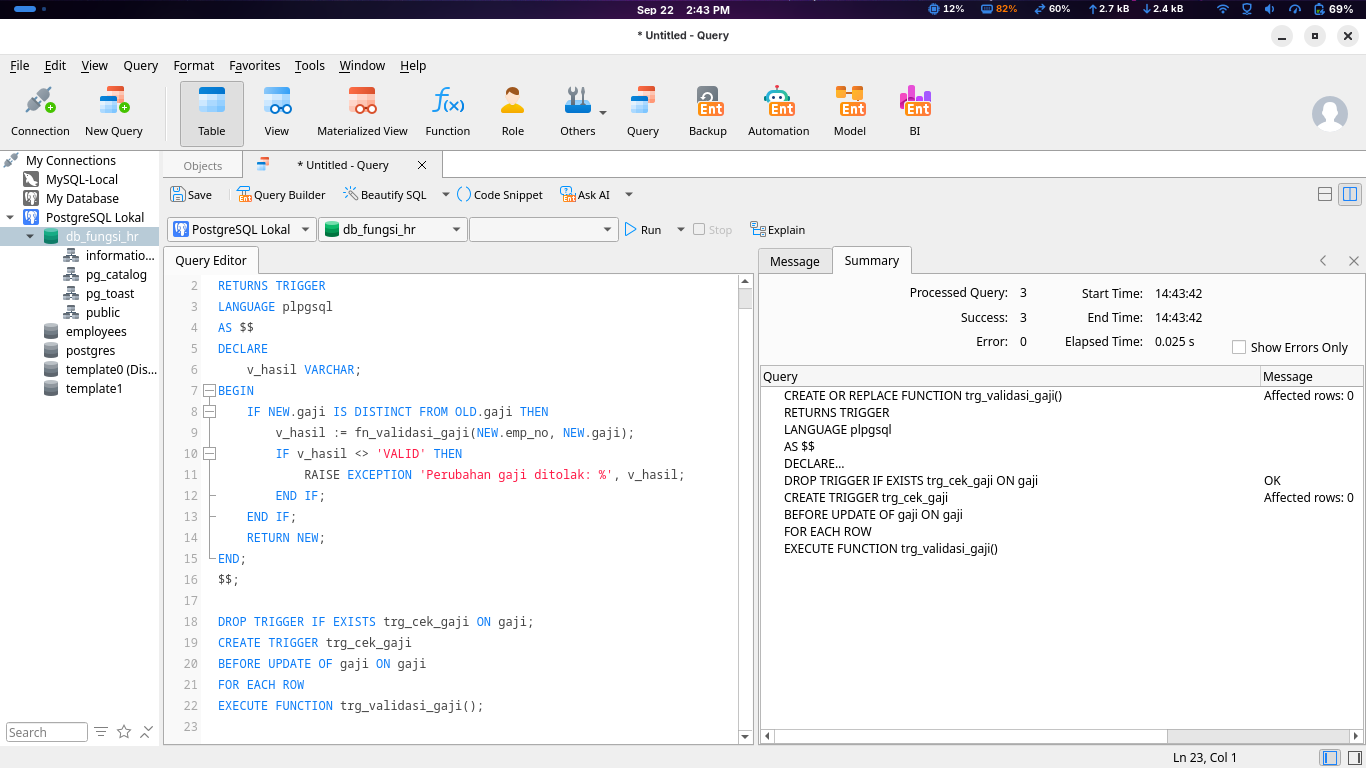
\includegraphics[width=0.9\textwidth,keepaspectratio]{ss_13_D5_trigger_buat.png}
\caption{Trigger trg\_cek\_gaji berhasil dibuat.}
\end{figure}
\begin{figure}[H]
\centering
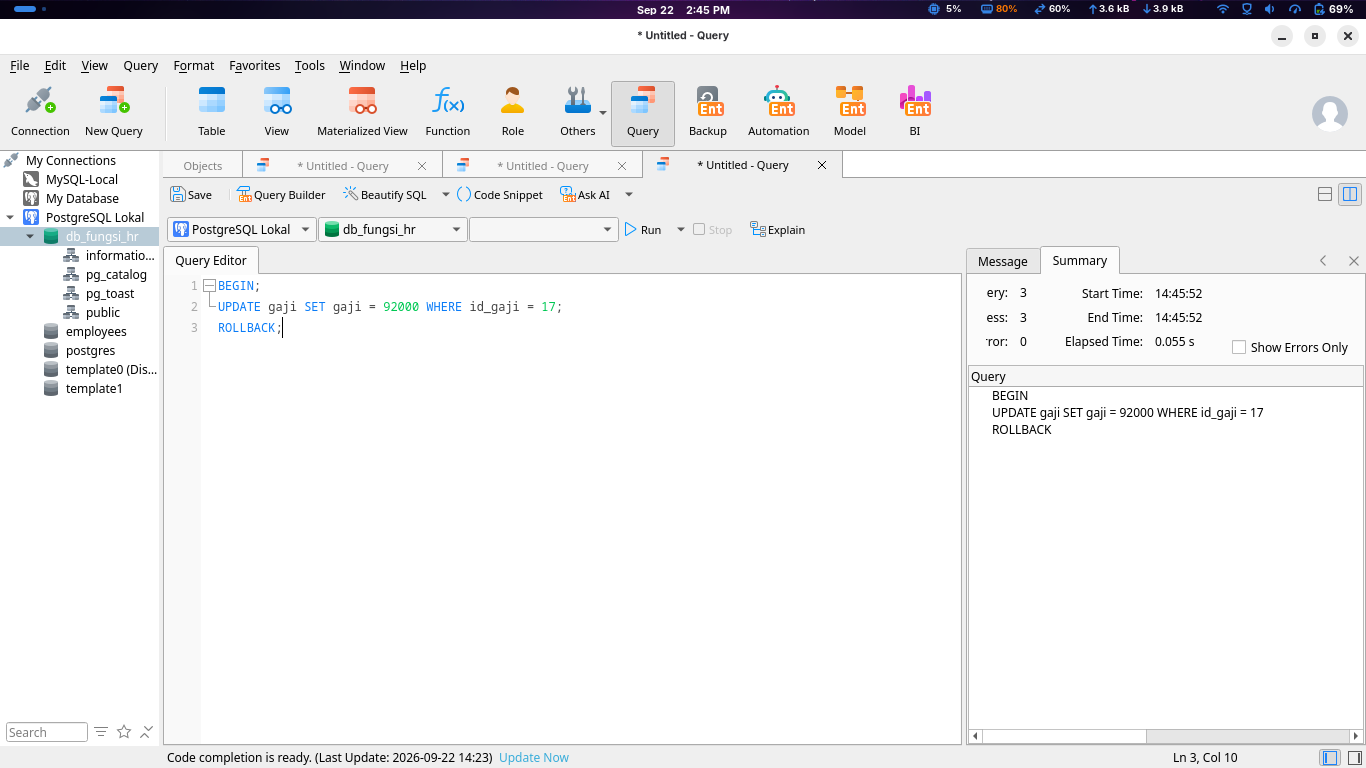
\includegraphics[width=0.9\textwidth,keepaspectratio]{ss_14_D5_trigger_uji.png}
\caption{Trigger menolak UPDATE tidak valid (ERROR) dan mengizinkan yang valid.}
\end{figure}
\smallskip
Trigger BEFORE UPDATE menolak perubahan bila hasil validasi bukan VALID (menggunakan RAISE EXCEPTION yang merupakan padanan SIGNAL SQLSTATE 45000).

\subsection*{D6. View}
\begin{figure}[H]
\centering
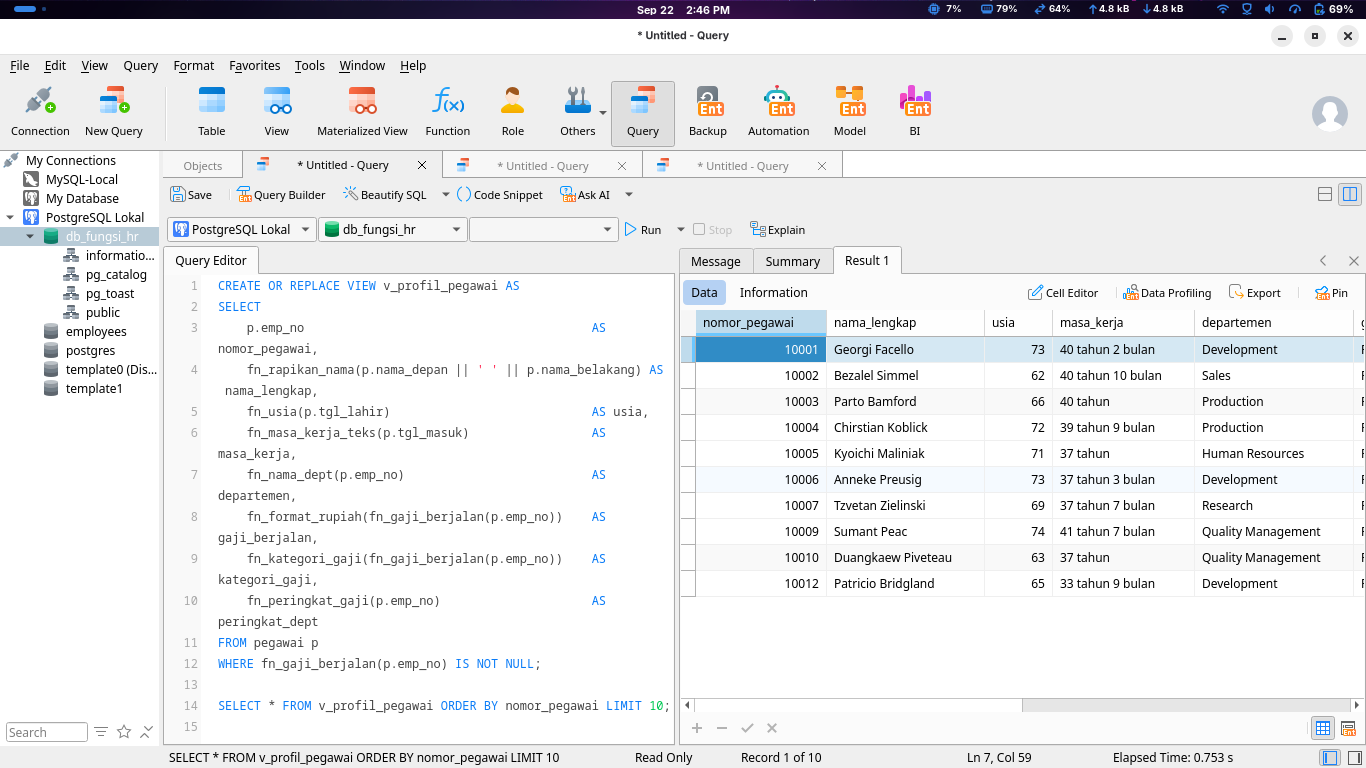
\includegraphics[width=0.9\textwidth,keepaspectratio]{ss_15_D6_view.png}
\caption{Pemanggilan view v\_profil\_pegawai (D6).}
\end{figure}
\smallskip
View membungkus query D1 sehingga cukup dipanggil dengan \texttt{SELECT * FROM v\_profil\_pegawai}.

\textbf{Analisis:} Fungsi terbaik untuk logika kompleks/bersyarat dengan parameter. View terbaik untuk presentasi berulang yang selalu live. Generated column terbaik untuk nilai turunan stabil yang sering difilter/disortir karena tersimpan fisik dan bisa diindeks.

\section*{E. Pengujian, Penelusuran, dan Pengelolaan}

\subsection*{E1. Inventaris Fungsi}
\begin{figure}[H]
\centering
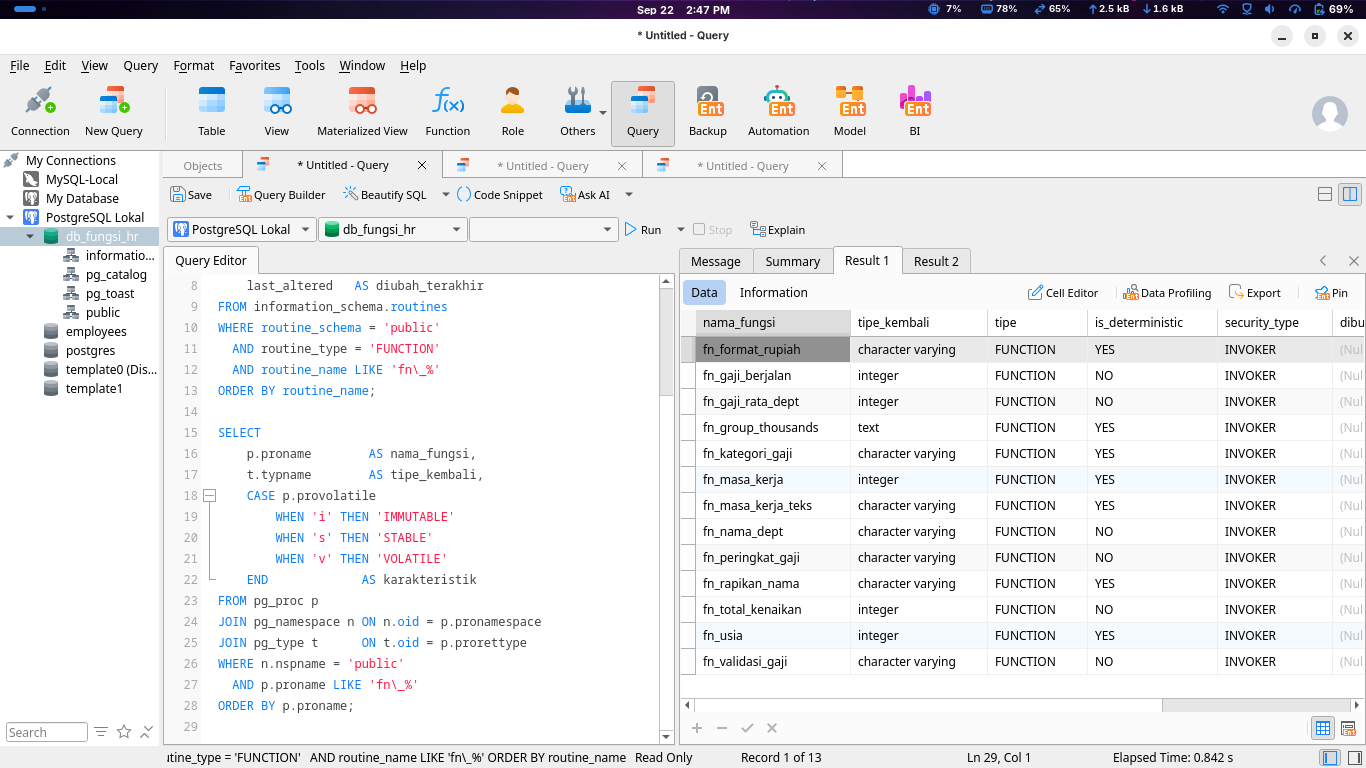
\includegraphics[width=0.9\textwidth,keepaspectratio]{ss_16_E1_inventaris.png}
\caption{Inventaris fungsi (E1).}
\end{figure}
\smallskip
Daftar seluruh fungsi buatan beserta tipe, determinisme, dan waktu pembuatan diambil dari information\_schema.ROUTINES dan pg\_proc.

\subsection*{E2. Pengujian Terpusat}
\begin{figure}[H]
\centering
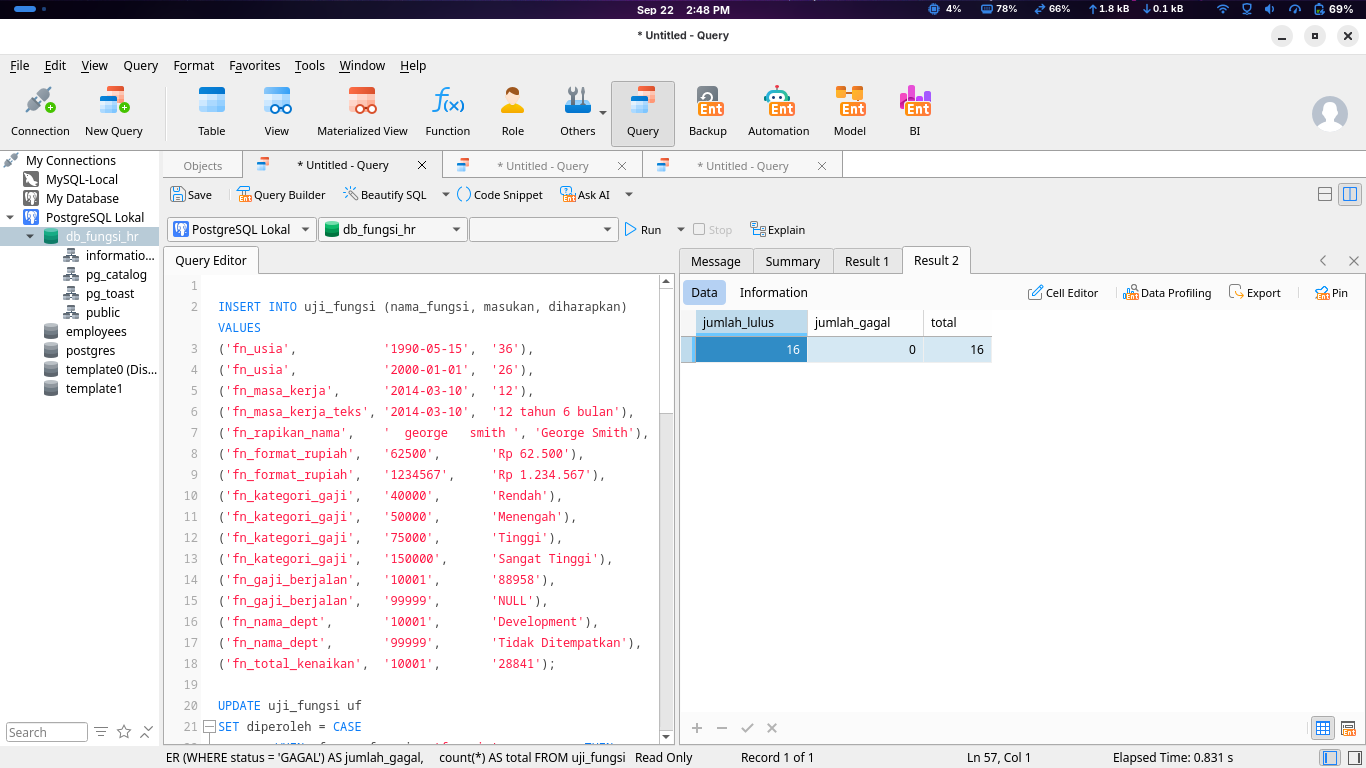
\includegraphics[width=0.9\textwidth,keepaspectratio]{ss_17_E2_uji.png}
\caption{Rekapitulasi hasil pengujian, 16 lulus dan 0 gagal (E2)}
\end{figure}
\smallskip
Enam belas kasus uji dicatat di tabel uji\_fungsi, dan seluruhnya LULUS.

\subsection*{E3. Penelusuran Galat}
\begin{figure}[H]
\centering
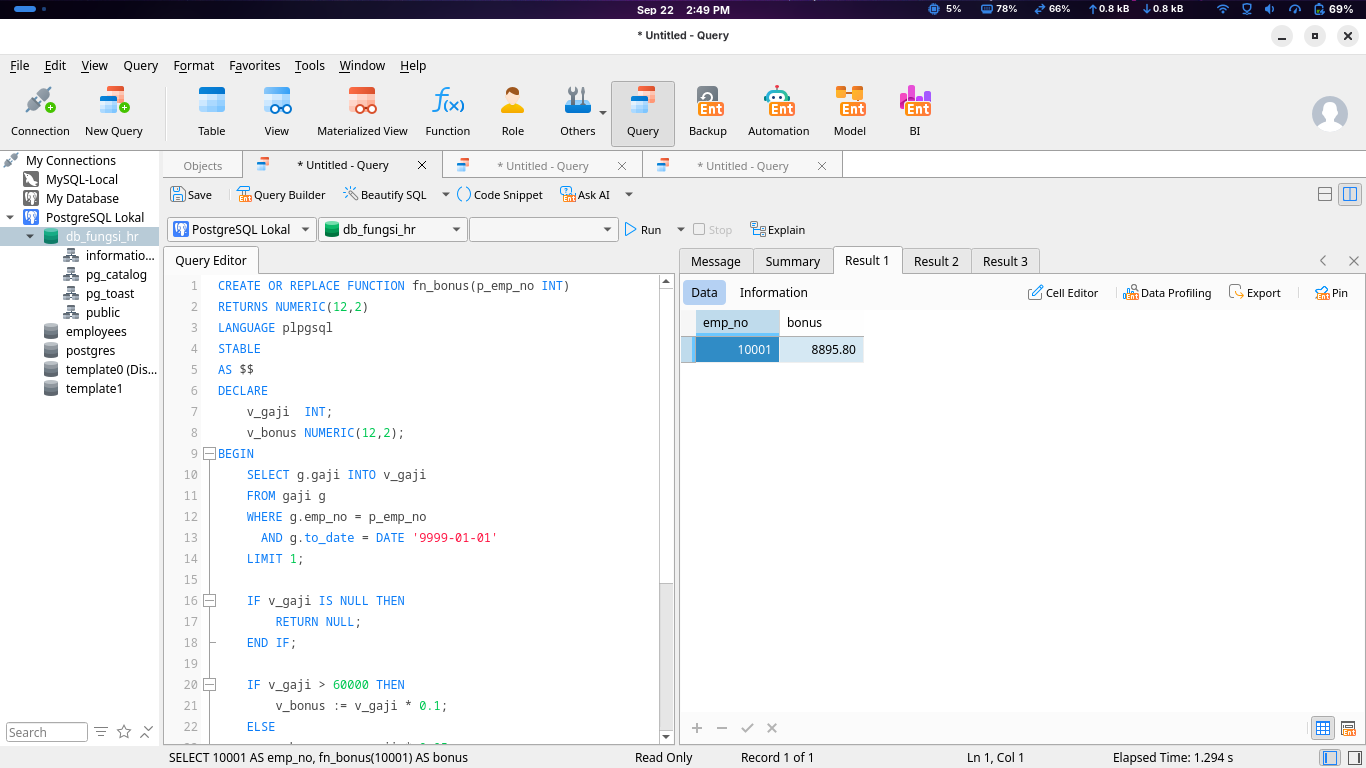
\includegraphics[width=0.9\textwidth,keepaspectratio]{ss_18_E3_debug.png}
\caption{Hasil fn\_bonus versi perbaikan (E3).}
\end{figure}
\smallskip
Skrip fn\_bonus yang diberikan mengandung enam kesalahan. Pertama, v\_bonus tidak dideklarasikan. Kedua, tidak ada RETURN. Ketiga, SELECT...INTO tanpa LIMIT (error bila lebih dari satu baris). Keempat, tidak menangani NULL pada v\_gaji. Kelima, pengali desimal pada variabel INT memotong presisi. Keenam, penggunaan DELIMITER yang tidak dikenali PostgreSQL. Versi perbaikan menghasilkan nilai bonus yang benar.

\textbf{Analisis:} Dua teknik penelusuran logika fungsi, yaitu RAISE NOTICE/INFO/DEBUG yang ringan namun keluaran masuk ke log dan bising bila berlebihan. Kedua, menyimpan jejak ke tabel audit yang lebih terstruktur namun menambah I/O dan bersifat efek samping (tidak cocok untuk fungsi IMMUTABLE/STABLE).

\subsection*{E4. Pengukuran Kinerja, Kolom vs Fungsi}
\begin{figure}[H]
\centering
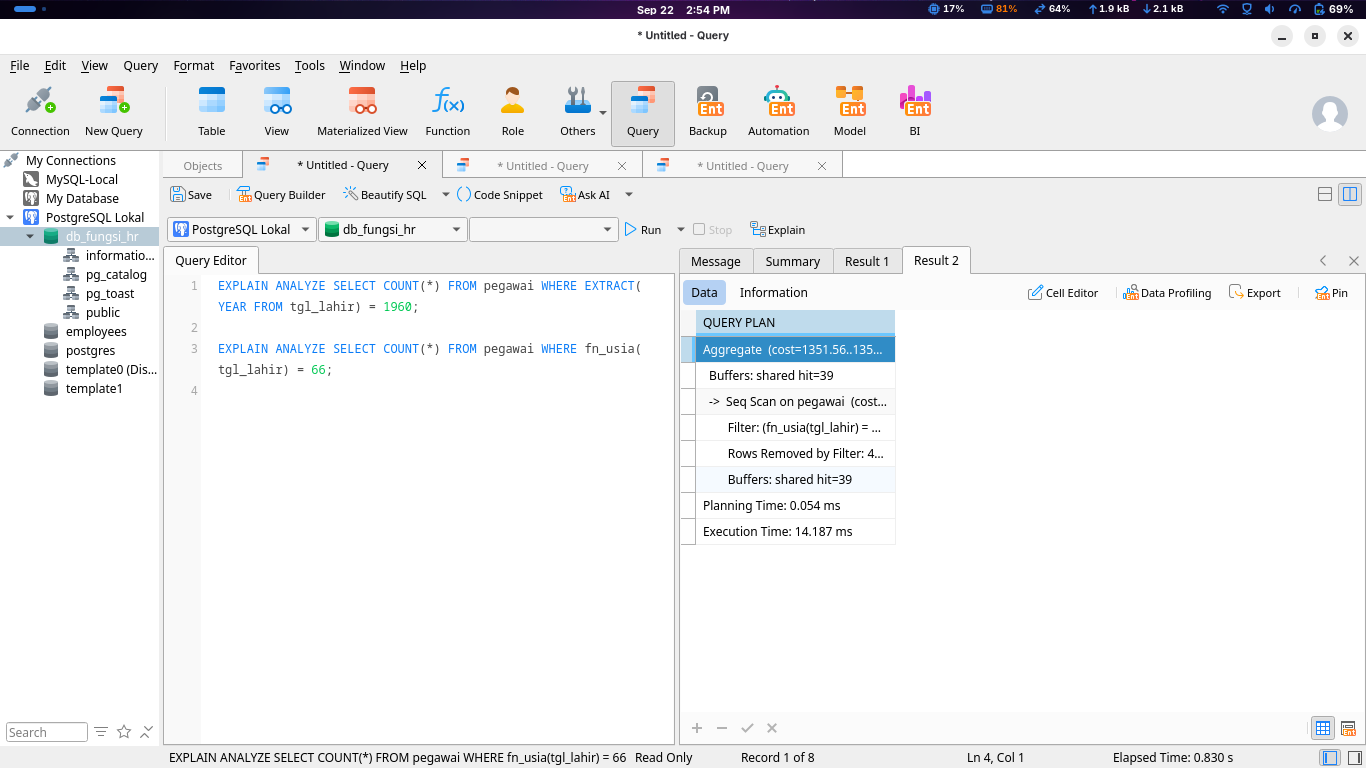
\includegraphics[width=0.9\textwidth,keepaspectratio]{ss_19_E4_benchmark.png}
\caption{Benchmark E4, kolom polos vs dibungkus fungsi}
\end{figure}
\smallskip
EXPLAIN ANALYZE membandingkan filter pada kolom polos versus kolom yang dibungkus fn\_usia.

\subsection*{E5. Pengukuran Kinerja, Fungsi vs JOIN}
\begin{figure}[H]
\centering
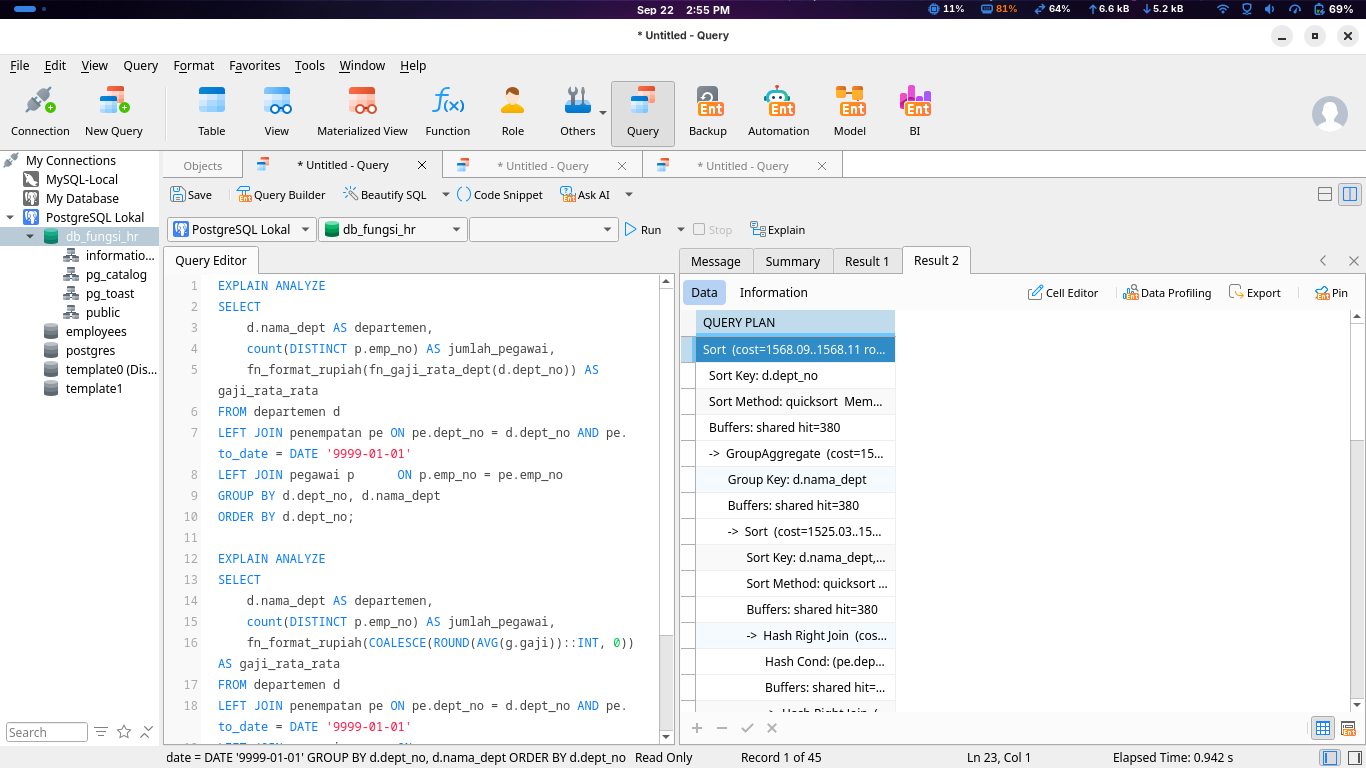
\includegraphics[width=0.9\textwidth,keepaspectratio]{ss_20_E5_benchmark.png}
\caption{Benchmark E5, fungsi vs JOIN+GROUP BY}
\end{figure}
\smallskip
EXPLAIN ANALYZE membandingkan rekap departemen yang memakai fn\_gaji\_rata\_dept versus versi JOIN + GROUP BY.

\textbf{Analisis:} predikat yang membungkus kolom dengan fungsi membuat indeks pada kolom mentah tidak terpakai (terjadi Seq Scan). Untuk tetap memakai indeks diperlukan expression index pada ekspresi tersebut. Perbandingan waktu eksekusi sebagai berikut

\begin{table}[H]
\centering
\caption{Perbandingan waktu eksekusi (E4 \& E5).}
\begin{tabular}{|l|r|r|}
\hline
\textbf{Ukuran} & \textbf{Langsung (kolom/JOIN)} & \textbf{Ber-fungsi}\\
\hline
E4 (filter 5.000 baris) & $\sim$2 ms  & $\sim$10 ms\\
E5 (rekap departemen)   & $\sim$24 ms & $\sim$78 ms\\
\hline
\end{tabular}
\end{table}

\subsection*{E7. Faktorial}
\begin{figure}[H]
\centering
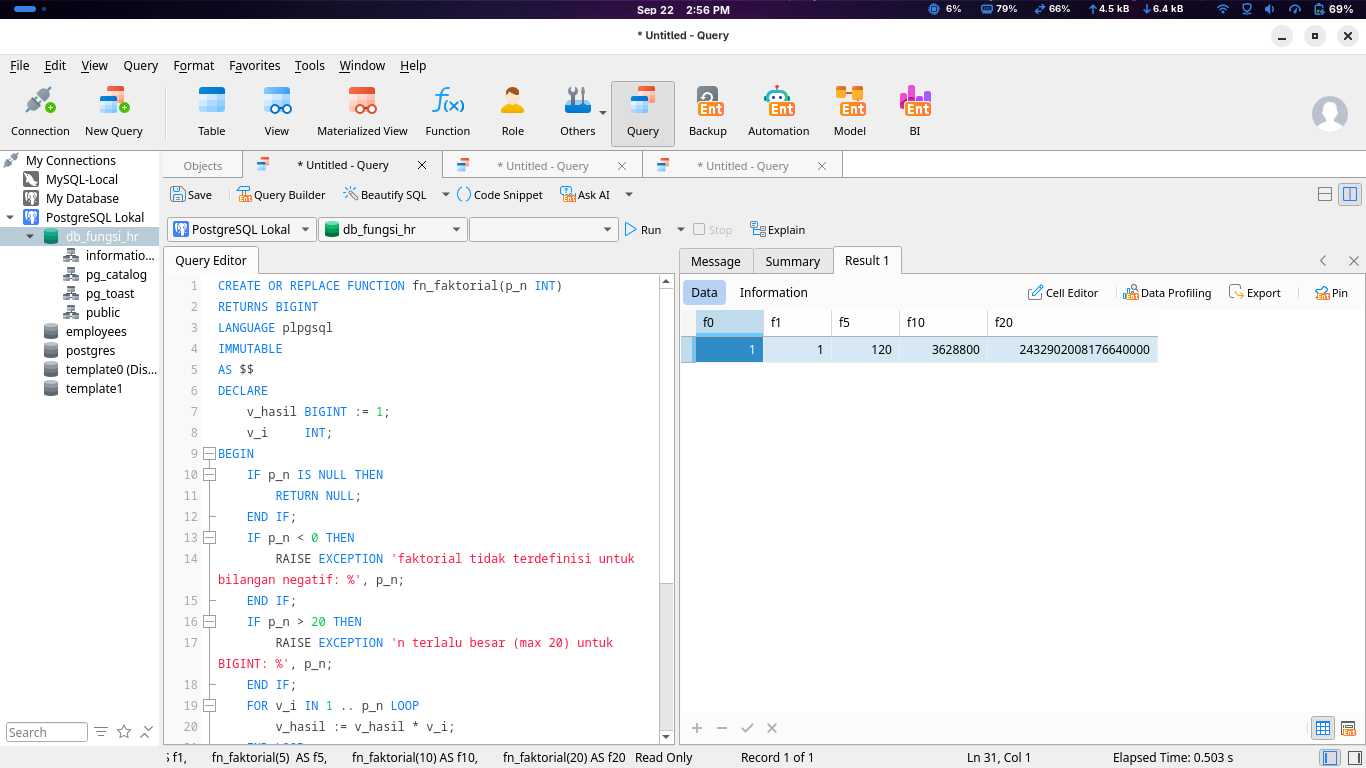
\includegraphics[width=0.85\textwidth,keepaspectratio]{ss_21_E7_faktorial.png}
\caption{Hasil fn\_faktorial (E7).}
\end{figure}
\smallskip
PostgreSQL (seperti MySQL) tidak mendukung rekursi fungsi, sehingga fn\_faktorial diimplementasikan dengan loop iteratif FOR.

\section*{Tugas Tambahan}

\subsection*{G1. Terbilang}
\begin{figure}[H]
\centering
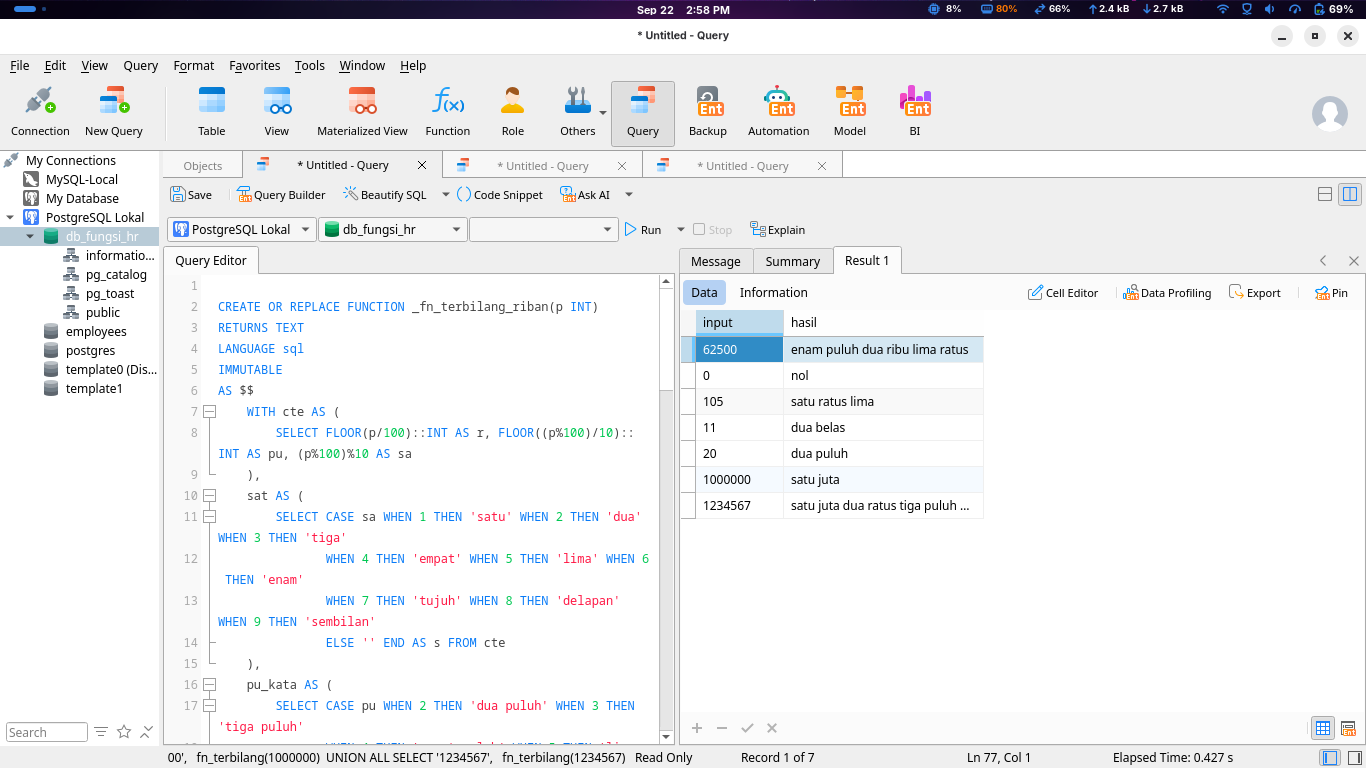
\includegraphics[width=0.9\textwidth,keepaspectratio]{ss_22_G1_terbilang.png}
\caption{Hasil fn\_terbilang (G1).}
\end{figure}
\smallskip
fn\_terbilang mengubah bilangan menjadi kata bahasa Indonesia sampai jutaan, misalnya 62500 menjadi ``enam puluh dua ribu lima ratus''.

\subsection*{G2. Hari Kerja}
\begin{figure}[H]
\centering
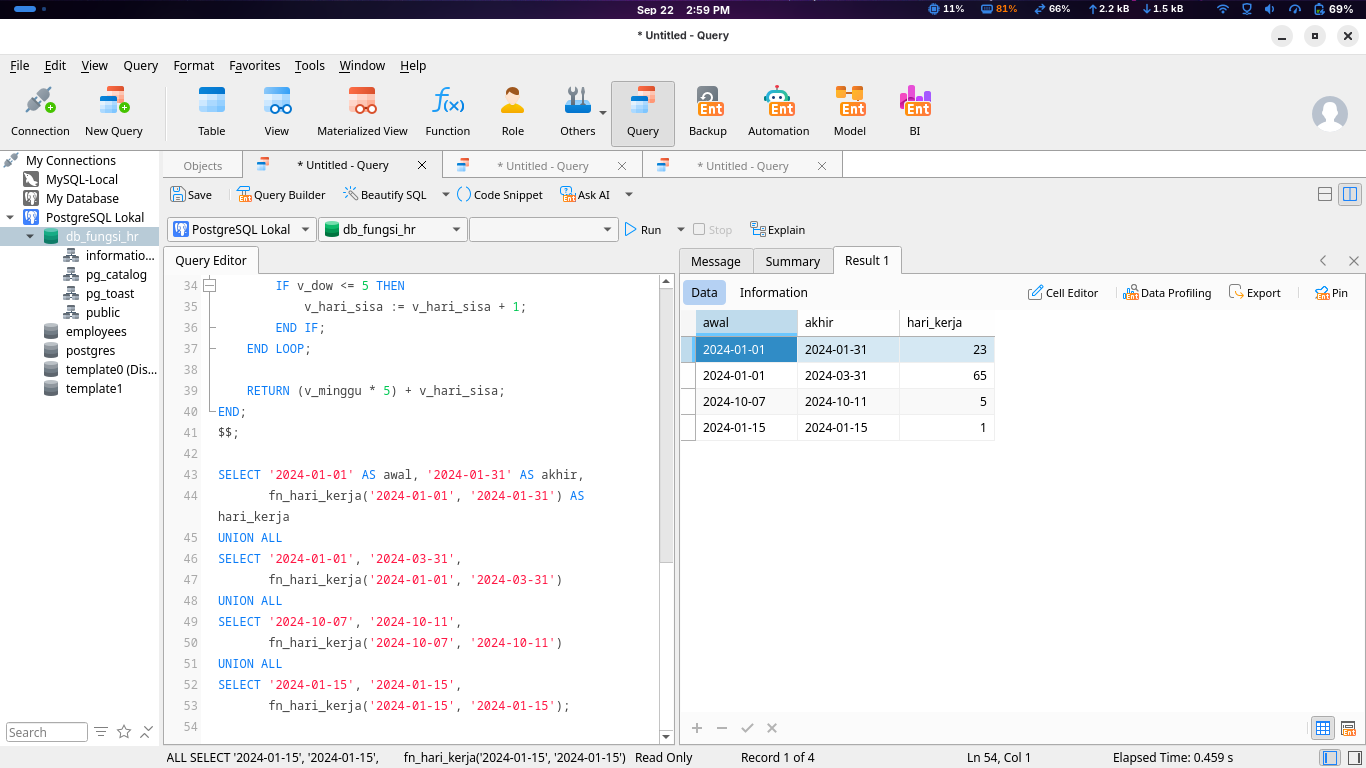
\includegraphics[width=0.9\textwidth,keepaspectratio]{ss_23_G2_hari_kerja.png}
\caption{Hasil fn\_hari\_kerja (G2).}
\end{figure}
\smallskip
fn\_hari\_kerja menghitung hari kerja dari Senin sampai Jumat antara dua tanggal dengan rumus matematis (minggu penuh $\times$ 5 + sisa), tanpa perulangan baris-per-baris.

\subsection*{G3. Caching}
\begin{figure}[H]
\centering
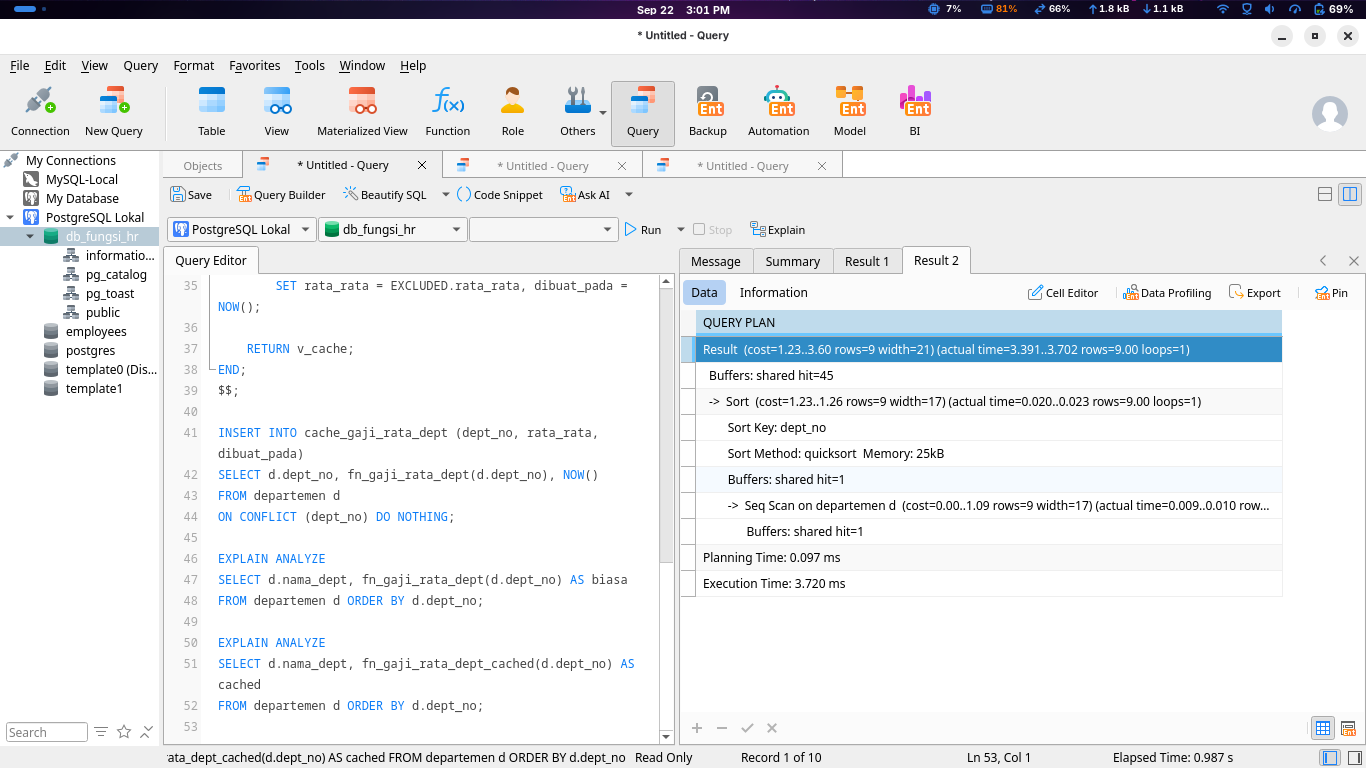
\includegraphics[width=0.9\textwidth,keepaspectratio]{ss_24_G3_caching.png}
\caption{Benchmark caching (G3), versi biasa vs versi cached}
\end{figure}
\smallskip
Mekanisme caching fn\_gaji\_rata\_dept memakai tabel cache\_gaji\_rata\_dept dengan masa kedaluwarsa 1 jam.

\textbf{Analisis:} caching mempercepat query secara signifikan (versi biasa $\sim$58 ms menjadi versi cached $\sim$1 ms pada data yang sama). Risikonya: bila data gaji berubah dalam jendela 1 jam, cache menyajikan nilai yang usang sampai kedaluwarsa. Untuk data yang berubah sering, kedaluwarsa perlu diperpendek atau cache di-invalidasi secara eksplisit.

\section*{Simpulan}
Fungsi basis data sangat berguna untuk menyusun logika bisnis yang berulang menjadi pendek, seragam, dan mudah dibaca. Praktikum ini membuktikan:
\begin{enumerate}
  \item Fungsi skalar murni (Bagian B) dan fungsi pembaca tabel (Bagian C) dapat dibuat, diuji, dan dirangkai secara berlapis dengan aman.
  \item Penerapan fungsi dalam skenario nyata (Bagian D) meliputi profil, validasi gaji, trigger, dan view. Semua berjalan sesuai ketentuan, dan trigger menolak perubahan yang tidak valid.
  \item Pengujian terpusat (E2) menunjukkan 16 dari 16 kasus LULUS.
  \item Fungsi yang membungkus kolom pada data besar menurunkan kinerja karena indeks tidak terpakai (Bagian E4 dan E5). Caching (G3) terbukti memberi percepatan signifikan.
\end{enumerate}
Tiga pedoman, yaitu gunakan fungsi untuk logika kompleks yang berulang. Kedua, hindari membungkus kolom dengan fungsi pada predikat query besar (gunakan expression index bila perlu). Ketiga, gunakan caching atau generated column untuk agregat berulang yang mahal.

\end{document}
